\documentclass[11pt]{article}
\usepackage[margin=1in]{geometry}
\usepackage{amsmath}
\usepackage{tikz}
\usepackage{pgfplots}
\pgfplotsset{compat=1.18}
\usetikzlibrary{arrows.meta,positioning,shapes.geometric,fit,backgrounds,calc,decorations.pathreplacing}
\usepackage{caption}

% ---- shared styles ----
\tikzset{
  blk/.style={rectangle, rounded corners=2pt, draw=black!70, thick, fill=blue!6,
              minimum height=8mm, minimum width=20mm, align=center, font=\small},
  io/.style={rectangle, rounded corners=6pt, draw=black!70, thick, fill=green!8,
             minimum height=8mm, align=center, font=\small},
  proc/.style={rectangle, draw=black!70, thick, fill=orange!10, minimum height=8mm,
               align=center, font=\small},
  dec/.style={diamond, aspect=2, draw=black!70, thick, fill=yellow!15, align=center, font=\footnotesize},
  ar/.style={-{Latex[length=2mm]}, thick},
  lbl/.style={font=\footnotesize\itshape, text=black!60},
}
\definecolor{good}{RGB}{34,139,34}
\definecolor{bad}{RGB}{178,34,34}
\definecolor{warn}{RGB}{218,165,32}

\begin{document}
\begin{center}\Large\textbf{ESA Phase-1 — Figure Set (TikZ)}\\[2pt]
\normalsize A Unified Benchmark for RL Post-Training of Language Models\end{center}
\vspace{1em}

% ============ FIG 1: system architecture ============
\begin{figure}[h]\centering
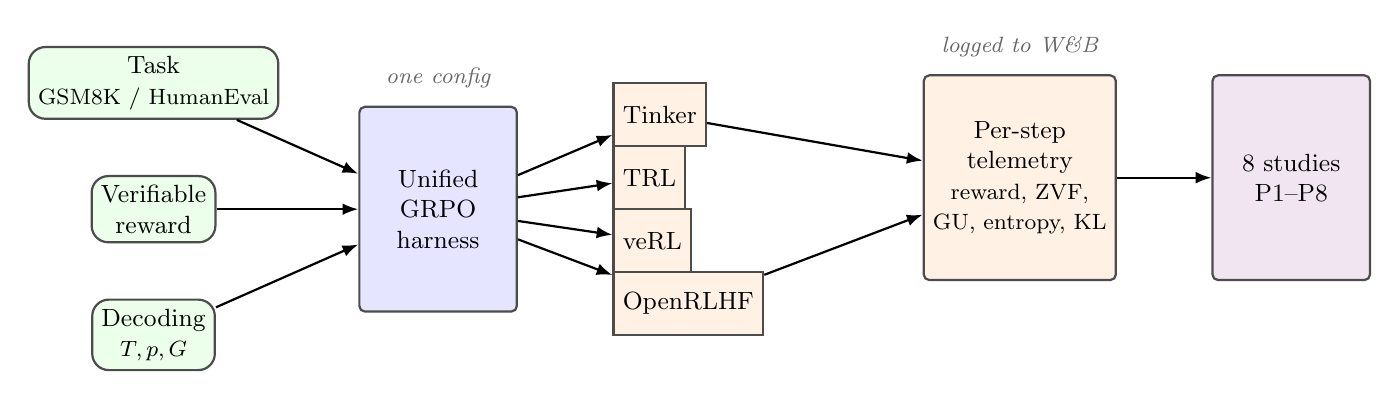
\begin{tikzpicture}[node distance=7mm and 12mm]
\node[io] (task) {Task\\\footnotesize GSM8K / HumanEval};
\node[io, below=of task] (rew) {Verifiable\\reward};
\node[io, below=of rew] (dec) {Decoding\\\footnotesize $T,p,G$};
\node[blk, right=18mm of rew, minimum height=26mm, fill=blue!10] (harness) {Unified\\GRPO\\harness};
\node[proc, right=of harness, yshift=12mm] (tk) {Tinker};
\node[proc, right=of harness, yshift=4mm] (trl) {TRL};
\node[proc, right=of harness, yshift=-4mm] (verl) {veRL};
\node[proc, right=of harness, yshift=-12mm] (orl) {OpenRLHF};
\node[blk, right=30mm of trl, fill=orange!10, minimum height=26mm] (tel) {Per-step\\telemetry\\\footnotesize reward, ZVF,\\ \footnotesize GU, entropy, KL};
\node[blk, right=of tel, fill=violet!10, minimum height=26mm] (studies) {8 studies\\P1--P8};
\foreach \s in {task,rew,dec} \draw[ar] (\s) -- (harness);
\foreach \d in {tk,trl,verl,orl} \draw[ar] (harness) -- (\d);
\draw[ar] (tk) -- (tel); \draw[ar] (orl) -- (tel);
\draw[ar] (tel) -- (studies);
\node[lbl, above=1mm of harness] {one config};
\node[lbl, above=1mm of tel] {logged to W\&B};
\end{tikzpicture}
\caption{System architecture: one task/reward/decoding config drives any framework backend; uniform per-step telemetry feeds the eight studies P1--P8. Differences are attributable to the \emph{stack}, not the experiment.}
\end{figure}

% ============ FIG 2: GRPO loop ============
\begin{figure}[h]\centering
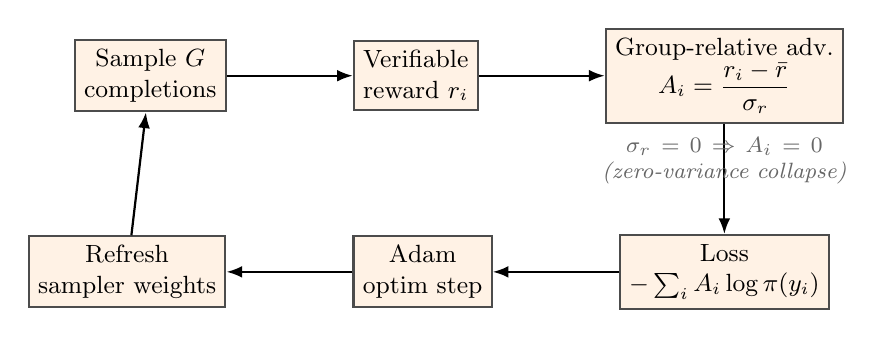
\begin{tikzpicture}[node distance=10mm and 16mm]
\node[proc] (samp) {Sample $G$\\completions};
\node[proc, right=of samp] (rew) {Verifiable\\reward $r_i$};
\node[proc, right=of rew] (adv) {Group-relative adv.\\$A_i=\dfrac{r_i-\bar r}{\sigma_r}$};
\node[proc, below=14mm of adv] (loss) {Loss\\$-\sum_i A_i\log\pi(y_i)$};
\node[proc, left=of loss] (opt) {Adam\\optim step};
\node[proc, left=of opt] (refresh) {Refresh\\sampler weights};
\draw[ar] (samp)--(rew); \draw[ar] (rew)--(adv); \draw[ar] (adv)--(loss);
\draw[ar] (loss)--(opt); \draw[ar] (opt)--(refresh); \draw[ar] (refresh)-- (samp);
\node[lbl, below=0.5mm of adv, text width=32mm, align=center] {$\sigma_r=0 \Rightarrow A_i=0$\\(zero-variance collapse)};
\end{tikzpicture}
\caption{The GRPO training loop as implemented on Tinker. When every completion in a group earns the same reward, $\sigma_r=0$, the advantage is identically zero, and the step contributes no gradient (the ZVF phenomenon quantified in P2).}
\end{figure}

% ============ FIG 3: ZVF collapse ============
\begin{figure}[h]\centering
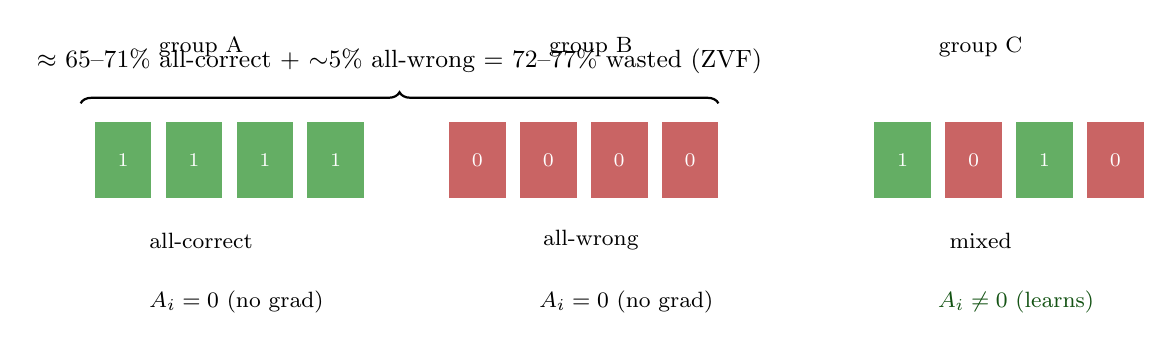
\begin{tikzpicture}[x=9mm,y=6mm]
\foreach \x/\v/\c in {0/1/good,1/1/good,2/1/good,3/1/good,
  5/0/bad,6/0/bad,7/0/bad,8/0/bad,
  11/1/good,12/0/bad,13/1/good,14/0/bad} {
  \fill[\c!70] (\x,0) rectangle (\x+0.8,1.6);
  \node[white,font=\scriptsize] at (\x+0.4,0.8) {\v};
}
\node at (1.5,3.2) {\footnotesize group A};
\node at (7,3.2) {\footnotesize group B};
\node at (12.5,3.2) {\footnotesize group C};
\node[font=\footnotesize] at (1.5,-0.9) {all-correct};
\node[font=\footnotesize] at (7,-0.9) {all-wrong};
\node[font=\footnotesize] at (12.5,-0.9) {mixed};
\node[font=\footnotesize] at (2,-2.2) {$A_i=0$ (no grad)};
\node[font=\footnotesize] at (7.5,-2.2) {$A_i=0$ (no grad)};
\node[font=\footnotesize,good!60!black] at (13,-2.2) {$A_i\neq 0$ (learns)};
\draw[decorate,decoration={brace,amplitude=4pt},thick] (-0.2,2.0)--(8.8,2.0);
\node[font=\small] at (4.3,2.9) {$\approx$ 65--71\% all-correct + $\sim$5\% all-wrong $=$ 72--77\% wasted (ZVF)};
\end{tikzpicture}
\caption{Zero-Variance Fraction (P2). Binary reward makes most groups collapse to all-correct (already-solved easy prompts) or all-wrong; only mixed groups carry gradient. Measured ZVF: 0.72--0.77 across four methods.}
\end{figure}

% ============ FIG 4: P1 per-layer grad norm (real data) ============
\begin{figure}[h]\centering
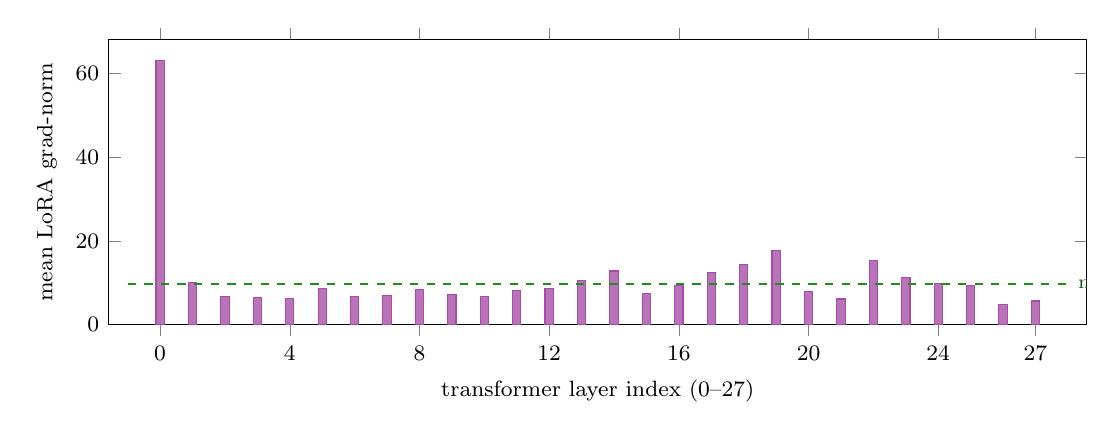
\begin{tikzpicture}
\begin{axis}[width=14cm,height=5.2cm,ybar,bar width=3pt,
  xlabel={transformer layer index (0--27)},ylabel={mean LoRA grad-norm},
  xmin=-1,xmax=28,ymin=0,ymax=68,enlarge x limits=0.02,
  xtick={0,4,8,12,16,20,24,27},tick label style={font=\footnotesize},
  label style={font=\footnotesize}]
\addplot[fill=violet!55,draw=violet!70] coordinates {
(0,63.03)(1,9.99)(2,6.65)(3,6.45)(4,6.27)(5,8.66)(6,6.64)(7,6.98)(8,8.36)(9,7.17)
(10,6.75)(11,8.22)(12,8.58)(13,10.47)(14,12.81)(15,7.50)(16,9.37)(17,12.35)(18,14.38)
(19,17.69)(20,7.88)(21,6.12)(22,15.26)(23,11.36)(24,9.88)(25,9.28)(26,4.79)(27,5.64)};
\draw[good,thick,dashed] (axis cs:-1,9.7)--(axis cs:28,9.7) node[right,font=\scriptsize,good!60!black]{mean};
\end{axis}
\end{tikzpicture}
\caption{P1 white-box (Colab L4, real data). Layer 0 dominates adaptation; a secondary mid--late band (layers 17--23) is active. Top 25\% of layers carry 47.6\% of gradient (moderate concentration --- which \emph{holds} at 3B, 0.39). At this toy scale the step-1 top-$k$ matched the final top-$k$ (overlap $=1.0$), but a scaled 3B/2-seed re-test drops this to $0.11$ (${\approx}$chance): predictability does \emph{not} survive scaling.}
\end{figure}

% ============ FIG 5: multi-seed campaign (real data) ============
\begin{figure}[h]\centering
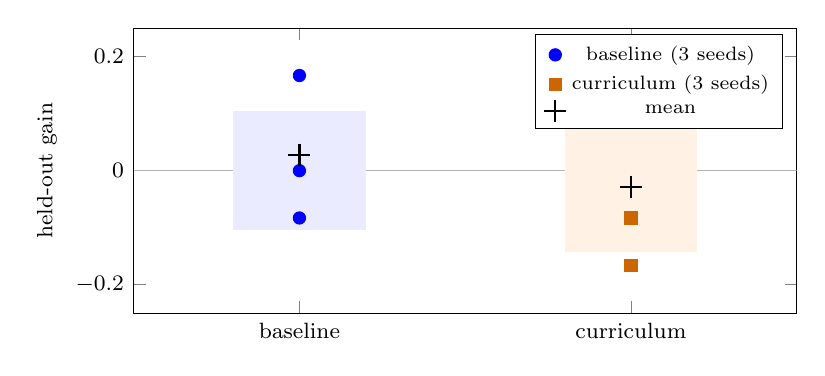
\begin{tikzpicture}
\begin{axis}[width=10cm,height=5.2cm,
  xtick={1,2},xticklabels={baseline,curriculum},xmin=0.5,xmax=2.5,
  ylabel={held-out gain},ymin=-0.25,ymax=0.25,
  tick label style={font=\footnotesize},label style={font=\footnotesize},
  legend style={font=\scriptsize,at={(0.98,0.98)},anchor=north east}]
\draw[black!30] (axis cs:0.5,0)--(axis cs:2.5,0);
% noise band +/- sd
\fill[blue!8] (axis cs:0.8,-0.104)rectangle(axis cs:1.2,0.104);
\fill[orange!10] (axis cs:1.8,-0.142)rectangle(axis cs:2.2,0.142);
\addplot[only marks,mark=*,blue,mark size=2.2pt] coordinates {(1,0.0)(1,0.167)(1,-0.083)};
\addplot[only marks,mark=square*,orange!80!black,mark size=2.2pt] coordinates {(2,0.167)(2,-0.083)(2,-0.167)};
\addplot[mark=+,mark size=4pt,black,thick,only marks] coordinates {(1,0.028)(2,-0.028)};
\legend{baseline (3 seeds),curriculum (3 seeds),mean}
\end{axis}
\end{tikzpicture}
\caption{Multi-seed campaign (real data). Per-seed held-out gains; shaded bands are $\pm 1$ sd. Baseline mean $+0.028$ vs curriculum $-0.028$ (difference $\approx 0.056$, SE $\approx 0.10$, $t\approx0.6$): \emph{no significant difference}, and curriculum costs $\sim$5--6$\times$ the sampling. The single-seed curriculum win ($+0.167$) was noise.}
\end{figure}

% ============ FIG 6: MIN-REPORT verifier flow ============
\begin{figure}[h]\centering
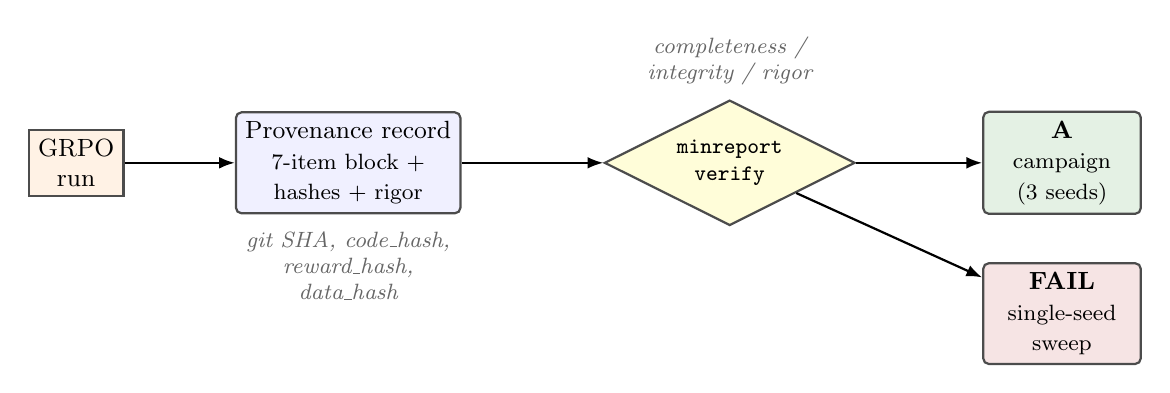
\begin{tikzpicture}[node distance=8mm and 14mm]
\node[proc] (run) {GRPO\\run};
\node[blk, right=of run] (rec) {Provenance record\\\footnotesize 7-item block +\\\footnotesize hashes + rigor};
\node[dec, right=18mm of rec, minimum width=22mm] (ver) {\texttt{minreport}\\\texttt{verify}};
\node[blk, right=16mm of ver, fill=good!12] (a) {\textbf{A}\\\footnotesize campaign\\\footnotesize (3 seeds)};
\node[blk, below=6mm of a, fill=bad!12] (f) {\textbf{FAIL}\\\footnotesize single-seed\\\footnotesize sweep};
\draw[ar] (run)--(rec); \draw[ar] (rec)--(ver);
\draw[ar] (ver)--(a); \draw[ar] (ver)--(f);
\node[lbl,above=0.5mm of ver,align=center,text width=30mm] {completeness /\\integrity / rigor};
\node[lbl,below=1mm of rec,align=center,text width=30mm] {git SHA, code\_hash,\\reward\_hash, data\_hash};
\end{tikzpicture}
\caption{P5 MIN-REPORT-RL verifier. Each run emits a signed provenance record; the verifier grades completeness (7 items), integrity (recomputes \texttt{code\_hash} vs live source), and rigor (hard-fails single-seed). It automatically flags the exact weakness kimi/codex caught by hand.}
\end{figure}

% ============ FIG 7: 8-pillar portfolio ============
\begin{figure}[h]\centering
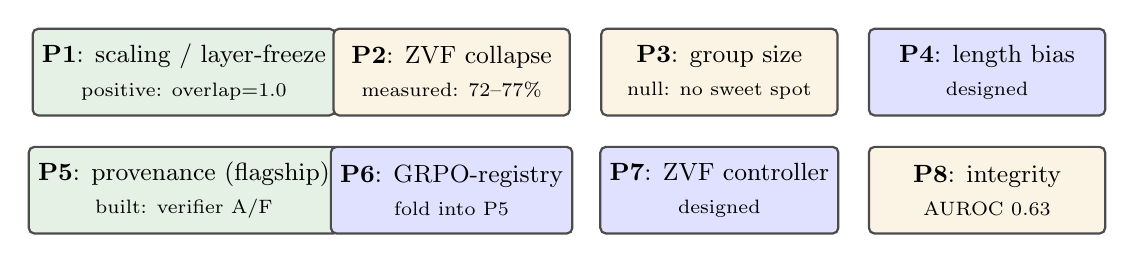
\begin{tikzpicture}[x=34mm,y=15mm,every node/.style={font=\footnotesize}]
\foreach \p/\x/\y/\name/\col/\st in {
 P1/0/1/{scaling / layer-freeze}/good/{positive: overlap=1.0},
 P2/1/1/{ZVF collapse}/warn/{measured: 72--77\%},
 P3/2/1/{group size}/warn/{null: no sweet spot},
 P4/3/1/{length bias}/blue/{designed},
 P5/0/0/{provenance (flagship)}/good/{built: verifier A/F},
 P6/1/0/{GRPO-registry}/blue/{fold into P5},
 P7/2/0/{ZVF controller}/blue/{designed},
 P8/3/0/{integrity}/warn/{AUROC 0.63}} {
  \node[blk, fill=\col!12, minimum width=30mm, minimum height=11mm] at (\x,\y)
    {\textbf{\p}: \name\\[1pt]\scriptsize \st};
}
\end{tikzpicture}
\caption{The eight-study portfolio and honest status. Strongest \emph{original} bets: P1 (predictive layer-freeze) and P5 (verifiable provenance). Green = positive/built, amber = measured/null, blue = designed.}
\end{figure}

% ============ FIG 8: P3 group-size (real data) ============
\begin{figure}[h]\centering
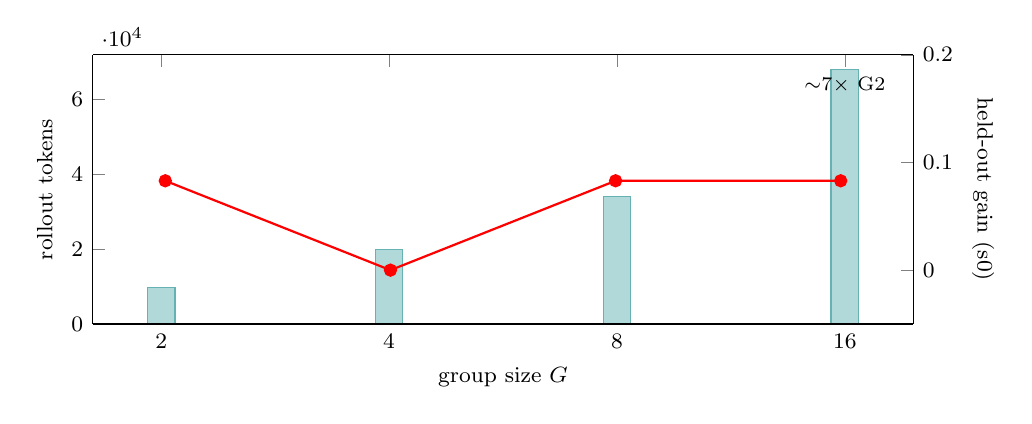
\begin{tikzpicture}
\begin{axis}[width=12cm,height=5cm,
  xlabel={group size $G$},ylabel={rollout tokens},
  xmode=log,log basis x=2,xtick={2,4,8,16},xticklabels={2,4,8,16},
  ymin=0,ymax=72000,tick label style={font=\footnotesize},label style={font=\footnotesize},
  axis y line*=left]
\addplot[fill=teal!30,draw=teal!60,ybar,bar width=10pt] coordinates {(2,9663)(4,19964)(8,34084)(16,68055)};
\node[font=\scriptsize] at (axis cs:16,64000){$\sim$7$\times$ G2};
\end{axis}
\begin{axis}[width=12cm,height=5cm,xmode=log,log basis x=2,xmin=1.6,xmax=20,
  ymin=-0.05,ymax=0.2,axis y line*=right,ylabel={held-out gain (s0)},
  xtick=\empty,tick label style={font=\footnotesize},label style={font=\footnotesize},
  y label style={rotate=180}]
\addplot[red,mark=*,thick] coordinates {(2,0.083)(4,0.0)(8,0.083)(16,0.083)};
\end{axis}
\end{tikzpicture}
\caption{P3 group size (real data, seed 0). Rollout tokens (bars) scale $\sim$linearly with $G$ (G16 $\approx7\times$ G2); held-out gain (red) shows \emph{no robust sweet spot} --- G4 was in fact the weakest single point. The earlier single-seed ``G=4 sweet spot'' claim does not survive.}
\end{figure}

\end{document}
